\documentclass{article}
\usepackage{graphicx}
\usepackage[top=1in, bottom=1in, left=1in, right=1in]{geometry}

\begin{document}

\title{Text Technologies for Data Science: Assessment 3}
\author{s1107496}

\maketitle

\section{Introduction}
This report describes the implementation of algorithms to detect duplicate (type 1), near duplicate (type 2), and number-heavy exact and near duplicate (type 3) news stories.

\section{Type 1 duplicate detection (task 2)}
Through manual examination, type 1 duplicates were determined to be exact duplicates. To detect these, a hash table with keys consisting of untokenized stories (with IDs removed) and values consisting of sets of story IDs was maintained. If, for a given key, there existed a matching story, the corresponding IDs were written to file. Otherwise, the story/ID key/value pair for the current line was written to the hash table.

\section{Type 2 duplicate detection (task 3)}
\subsection{Implementation overview}
To detect type 2 duplicates, stories were first tokenized by splitting on whitespace and other non-alphanumeric characters, using the regular expression suggested by Victor Lavrenko. Stories that had already been detected as type 1 duplicates were skipped. Stopwords, as given by \texttt{nltk}, were filtered out before frequencies for each token were computed. A simhash implementation using the md5 hashing algorithm from \texttt{hashlib} was then used to find potential duplicates, with tokens weighted by frequency. A difference metric between these potential duplicates was then computed by subtracting the size of the union of their token sets from the size of the intersection of their token sets; the first (if any) duplicate with fewer than three differences was written to file.
\subsection{\texttt{K} and \texttt{L} optimization}
While the initial values of 33 and 3 chosen for \texttt{K} and \texttt{L} (respectively) achieved 100\% recall on data.train, these values resulted in a running time on data.test of over 30 minutes. To remedy this, values for \texttt{K} and \texttt{L} were hand-optimized to maximize expected recall on data.test (see figure below). With \texttt{K} set to 28 and \texttt{L} set to 1, 66.67\% of items from data.train were correctly retrieved, while also processing XXX\% of data.test within 30 minutes (as measured on a DICE machine with an i5 processor and 8GB RAM).
\begin{figure}[ht!]
\centering
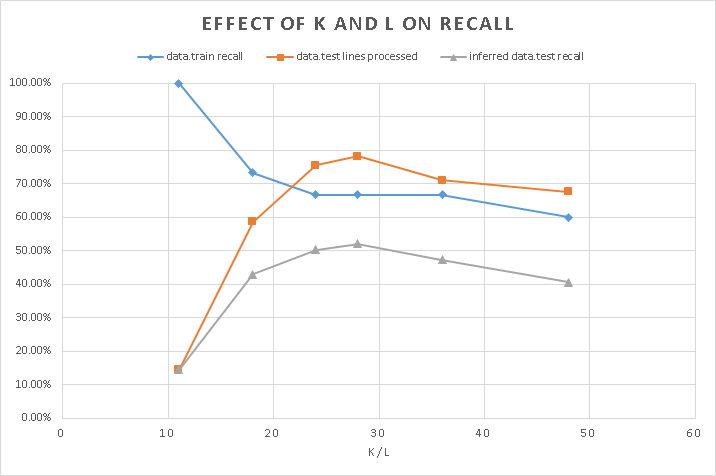
\includegraphics[width=165mm]{graph.png}
(Tests run on computer with an i5 processor and 24GB RAM.)
\end{figure}

\section{Type 3 duplicate detection (task 5)}
Type 3 duplicates were considered to be type 1 or type 2 duplicates found in number-heavy sections of stories, as detected via Finn's method. Type 3 duplicate detection was run directly before type 1 and 2 detection, to allow the latter to run up to the 30 minute time limit. Finn's method was implemented using the linear-time algorithm presented in the Text Technologies lecture, with \texttt{c} set to 100 as prescribed. This was performed on token sets before attempting any further duplicate detection. For type 3 detection, \texttt{K} was set to 33 and \texttt{L} was set to 3, as these settings had yielded accurate results for type 1 and 2 detection, but duplicate detection methods were otherwise unchanged from those used to identify type 1 and 2 duplicates. 72 instances of type 3 duplicates were detected.

\end{document}